\documentclass{beamer}
\usepackage{tikz}
\usetheme{Madrid}
\usepackage{ctex}
\usecolortheme{default}
\usepackage{verbatim}
\title[2022.12.26日汇报] %optional
{2022.12.26汇报}
%\subtitle{Demonstrating the Berkeley theme}
\author[周添文] % (optional)
{周添文\inst{} }

\institute[] % (optional)
{
  \inst{}%
  数学科学学院\\
  北京师范大学\\
 % \and
  %\inst{2}%
%  Faculty of Chemistry\\
%  Very Famous University
}

\date[2022.12.26] % (optional)
%{Very Large Conference, April 2021}

% Use a simple TikZ graphic to show where the logo is positioned

%\node[draw,color=white] at (0,0) {LOGO HERE};


%End of title page configuration block
%------------------------------------------------------------
%The next block of commands puts the table of contents at the 
%beginning of each section and highlights the current section:

\AtBeginSection[]
{
  \begin{frame}
    \frametitle{Table of Contents}
    \tableofcontents[currentsection]
  \end{frame}
}
%------------------------------------------------------------
\begin{document}
\frame{\titlepage}
%\logo{\includegraphics[]{bnu.png}}
%---------------------------------------------------------
%Highlighting text
\begin{frame}
\frametitle{图像去遮挡(Obstruction)算法}
本文主要研究去除图像中遮挡物的算法,其中,遮挡物可以是多种多样的,其大致可分为可反射(如玻璃)的和不透明的(如栅栏)等。\pause

在图像拍摄过程中,我们要求对同一场景拍摄不同角度的多张照片(类似全景照片),同时,要求场景中的\textbf{每一个像素至少可以在一帧照片中是不被遮挡的}。
\end{frame}
\begin{frame}
\frametitle{符号规定}
我们将一个标量记作小写字母$a$, 将一个向量记作大写字母$A$, 将一个矩阵记作粗体的大写字母$\textbf{A}$, 用$A\circ B$表示两个向量的内积。
\end{frame}
\begin{frame}
\frametitle{图像的分解}
将拍摄到的图像记作$I\in\mathbb{R}^n$,我们可以将其分解为
\begin{equation}
I = I_O + A(I_B - I_O)
\end{equation}
即为
\begin{equation}
I = (1-A)I_O+AI_B
\end{equation}
其中,向量$I_O\in \mathbb{R}^n$代表遮挡层,$n$代表像素数量,$I_B\in \mathbb{R}^n$代表真实的背景图像,$A\in \mathbb{R}^n$是$\alpha$混合掩膜(alpha blending mask)\pause

注:Alpha blending是将半透明的前景色与背景色结合的过程,可以得到混合后的新颜色。一幅彩色图像的每个像素用R,G,B三个分量表示,若每个分量用8位,那么一个像素共用3X8=24位表示。 在用32位表示一个像素时,若R,G,B分别用8位表示,剩下的8位常称为\textbf{α通道(alpha channel)位}。它用来表示该像素如何产生\textbf{半透明效果}。alpha的取值一般为0到255。 为0时,表示是全透明的,即图片是看不见的。为255时,表示图片即为原始图像。而中间的任意值即为半透明状态。
\end{frame}
\begin{frame}
\frametitle{图像的分解}
分解式
\begin{equation}
I = (1-A)I_O+AI_B
\end{equation}
中,$A\circ I_B$表明对背景图像$I_B$与$A$做向量内积,也就是将其作用在背景图像的每一个像素上\pause

特别地,如果遮挡物是一个可以反射的物体,则由于玻璃等常见反射物都是各向同性的(Homogeneous)。因此,我们可以认为这种情况下的$A$是常值向量。
\end{frame}
\begin{frame}
\frametitle{图像的分解}
显然,由于计算机并不能自动区分背景和遮挡物,因此,只针对一张图片是无法进行上述分解的。\pause

故在拍摄过程中,我们要求拍摄者移动相机,拍下多张图片。在移动过程中,由于遮挡物一般距离镜头较近,而背景距离镜头较远,因此遮挡物在不同照片中的移动距离会比背景更显著。利用这一差异,我们尝试区分开遮挡物和背景。
\end{frame}
\begin{frame}
\frametitle{预期效果}
\begin{figure}[!h]
\centering
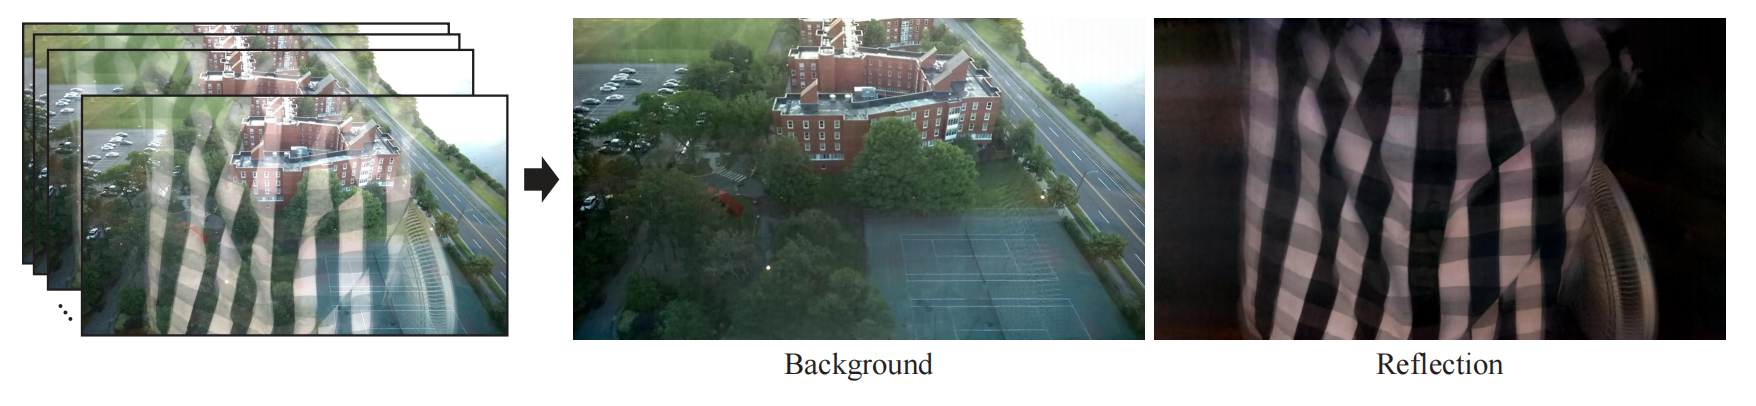
\includegraphics[height=2.5cm,width=10cm]{2022121601.png}
\caption{效果图1}
\end{figure}
\begin{figure}[!h]
\centering
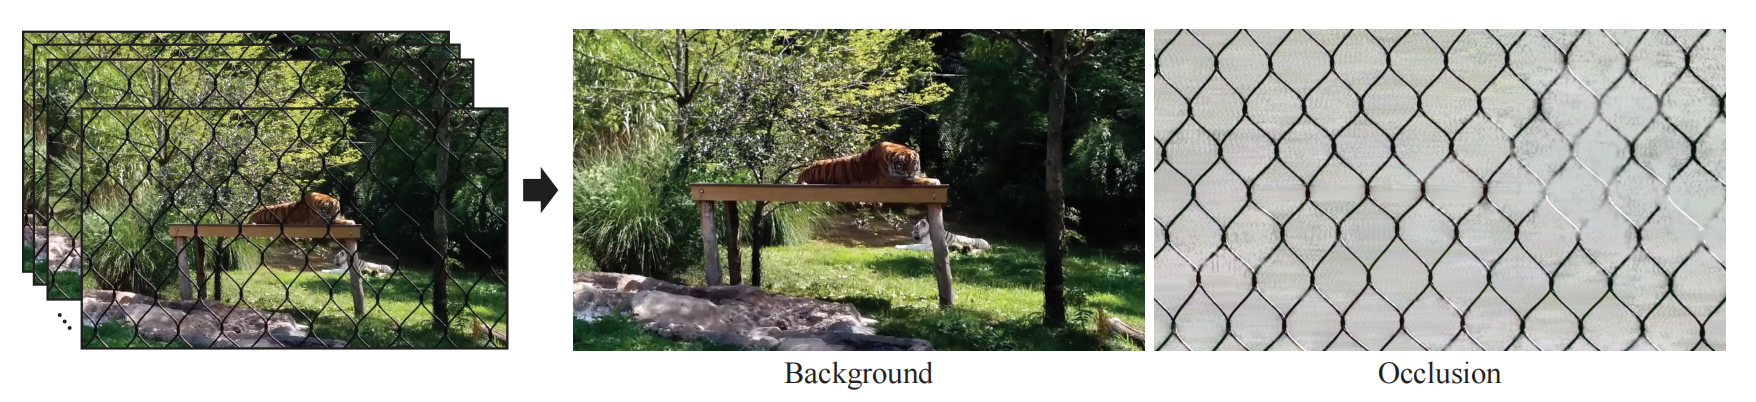
\includegraphics[height=2.5cm,width=10cm]{2022121602.png}
\caption{效果图2}
\end{figure}
\end{frame}
\begin{frame}
\frametitle{具体操作}
对于拍摄的一组图像,我们(任意)选取一帧图像作为参考帧,记作$t_0$,尝试利用其他帧$t$的信息估计$t_0$帧所对应的$I_B$和$I_O$.\pause

记$V^t_O$,$V^t_B$为第$t$帧中,障碍物和背景所对应的运动场(motion fields)\footnote{三维速度矢量在图像平面上的映射}\pause

由于打印出来的照片一般都是不平的,因此其可以看作参考帧$t_0$经过一定扭曲(wrap)后形成的图像。记$\textbf{W}(V_B^t)\in\mathbb{R}^{n\times n}$为图像的扭曲矩阵,则$\textbf{W}(V_B^t)I_B$即为背景图像$I_B$扭曲后的结果。\pause

因此,第$t$帧的图像可以表示为:
\begin{equation}
I^t = (1-\textbf{W}(V_O^t)A)\circ\textbf{W}(V_O^t)I_O+W(V_O^t)A\circ\textbf{W}(V_B^t)I_B
\end{equation}
\end{frame}
\begin{frame}
\frametitle{扭曲矩阵}
图像的扭曲(wrap)可以看作图像定义域改变的过程,其均可以通过矩阵进行描述

\begin{figure}[!h]
\centering
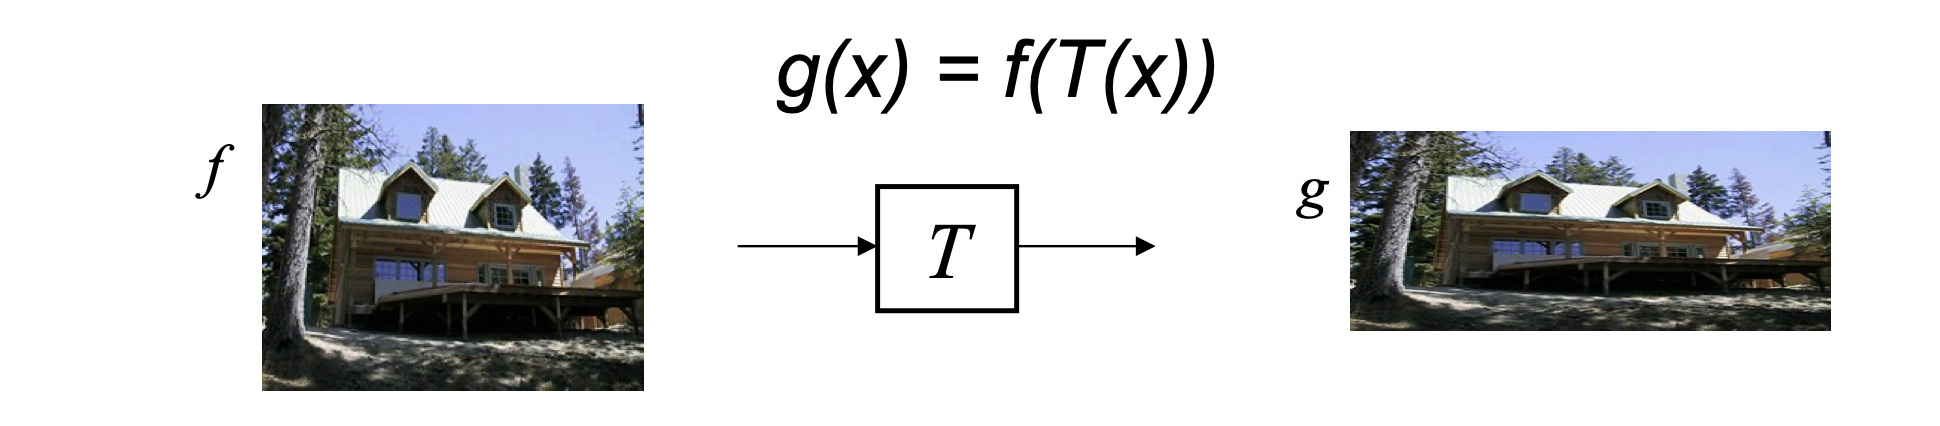
\includegraphics[height=2cm,width=10cm]{2022122601.png}
\caption{图像扭曲}
\end{figure}
\end{frame}
\begin{frame}
\frametitle{不同类型的图像扭曲}
\begin{figure}[!h]
\centering
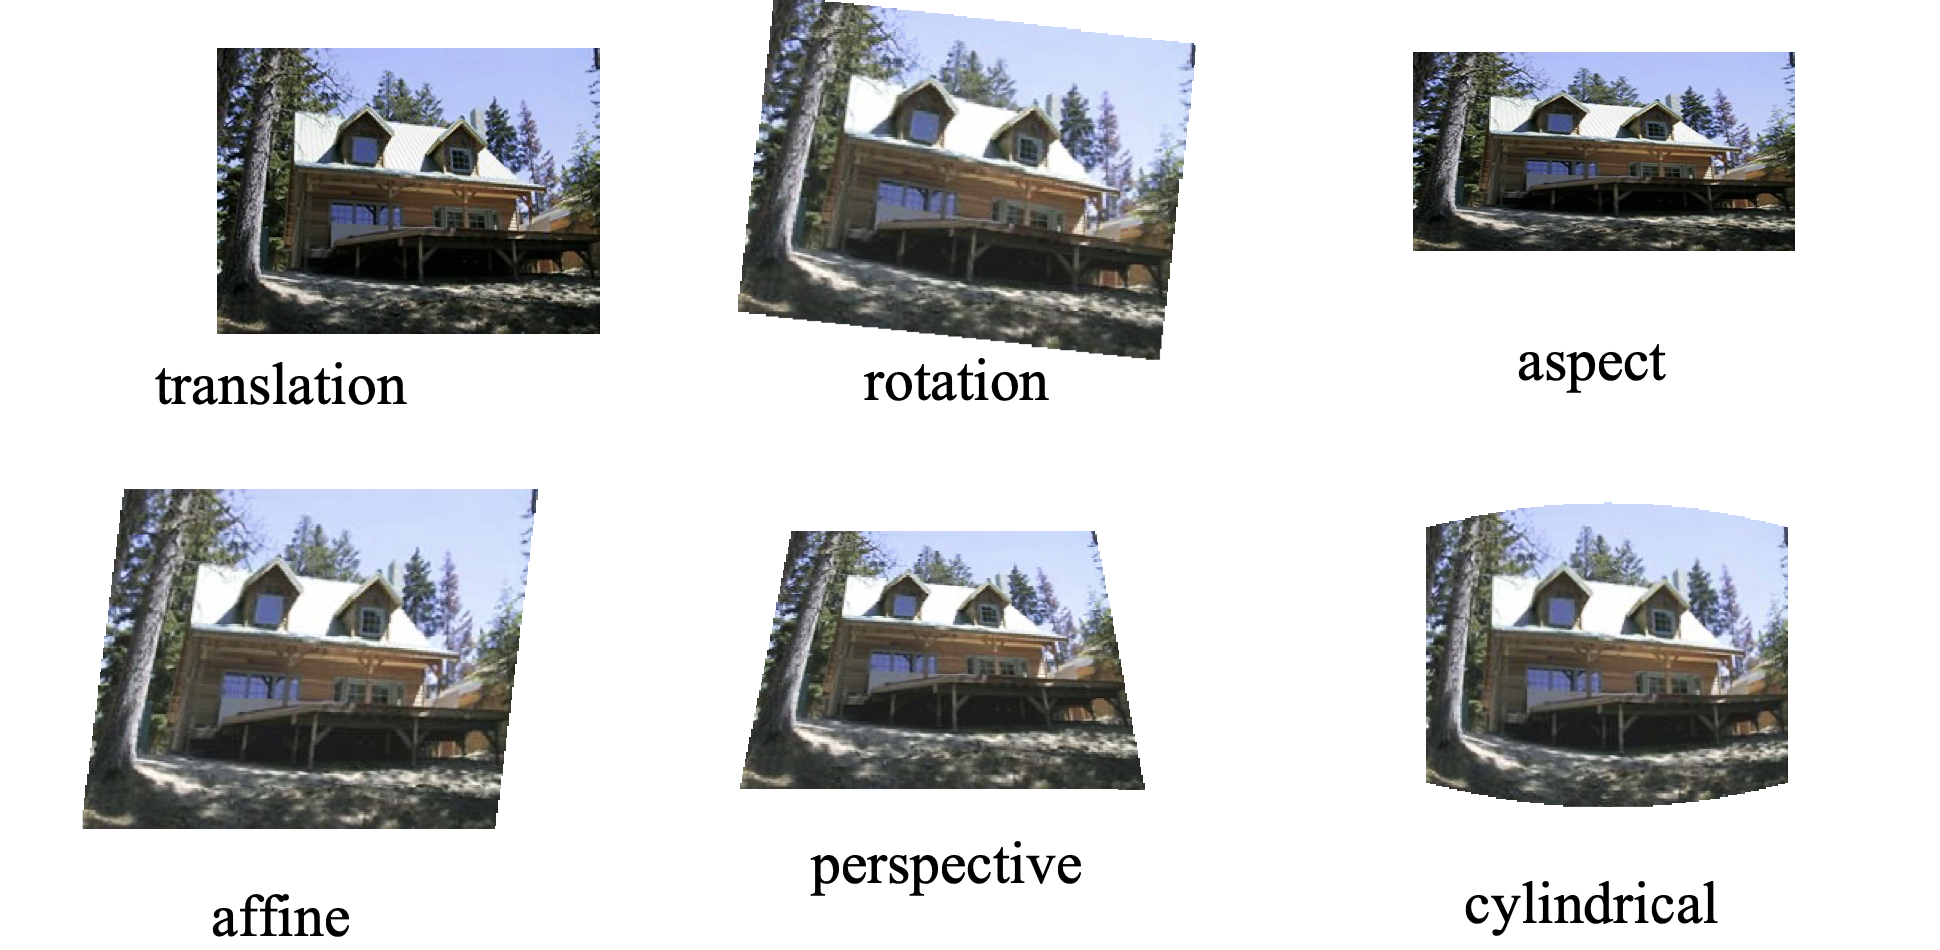
\includegraphics[height=4cm,width=10cm]{2022122602.png}
\caption{不同类型的图像扭曲}
\end{figure}
\end{frame}
\begin{frame}
\frametitle{具体操作}
由于$\alpha$混合掩膜是由障碍物产生的,因此,$\alpha$混合掩膜的运动状态与障碍物$I_O$相同,与背景$I_B$无关。\pause

因此,我们可以进行如下化简:

将$(1-A)\circ I_O$简记作$I_O$,原方程可化简为:
\begin{equation}
I^t = \textbf{W}(V_O^t)(1-A)\circ\textbf{W}(V_O^t)I_O+W(V_O^t)A\circ\textbf{W}(V_B^t)I_B
\end{equation}
\begin{equation}
=\textbf{W}(V_O^t)I_O+W(V_O^t)A\circ\textbf{W}(V_B^t)I_B
\end{equation}\pause
特别而言,由前所述,在反射的情况中,$\alpha$混合掩膜是常数$A=\alpha$,因此我们可以记$I_B = \alpha I_B$,且$W(V_O^t)A = \alpha$

进而,上式可以化简为
\begin{equation}
I^t = \textbf{W}(V_O^t)I_O+\textbf{W}(V_B^t)I_B
\end{equation}\pause
因此,我们的目标即为根据参考帧$t_0$以及图像序列${I^t}$的信息,在不知道运动场$V_B^t$,$V_O^t$以及$A$的情况下,确定背景$I_B$和$I_O$.
\end{frame}
\begin{frame}
\frametitle{基于运动进行分解}
由上文,在一般情况下,$A$并不是常数,因此我们将先讨论$A$随空间位置变化的情况:

由前文中的图像分解方程,我们可以设置数据项(data term)为:
\begin{equation}
\Sigma_t ||I^t-\textbf{W}(V_O^t)I_O-W(V_O^t)A\circ\textbf{W}(V_B^t)I_B||_1
\end{equation}
除此以外,由文献[1],由于背景图像是自然景象,我们知道$I_O$和$I_B$的梯度符合重尾分布
\begin{equation}
||\nabla I_O||_1+||\nabla I_B||_1
\end{equation}
\end{frame}
\begin{frame}
\frametitle{基于运动进行分解}
又由于$\alpha$映射通常比自然图像更加平滑,因此,我们认为其梯度应该遵循高斯分布,且对其$l_2$范数进行限制(penalize)
\begin{equation}
||\nabla A||^2
\end{equation}\pause
除此以外,由于背景图像和障碍物大多时候是独立存在的。因此,如果在输入的图像上出现了较大的梯度变化,我们认为是二者之中的一个所导致的,而不是二者一起导致的,因此,我们还需要施加下述限制:
\begin{equation}
L(I_O,I_B) = \Sigma_x ||\nabla I_O(x)||^2||\nabla I_B(x)||^2
\end{equation}
其中,$x$为空间索引,即空间位置坐标,$\nabla I_B(x)$是图像$I_B$在点$x$处的梯度
\end{frame}
\begin{frame}
\frametitle{基于运动进行分解}
由于两帧照片之间的时间间隔较短,因此,当运动比较细微时,光流(物体所成像的瞬时速度)可以用一阶Taylor展开式写作:
\begin{equation}
I_xu+I_yv+I_t = 0
\end{equation}
其中,$I_x$,$I_y$,$I_t$是图像$I(x,y,t)$的一阶偏导数,$(u,v)$是光流的位置向量。\pause

在我们的问题中,可以记作下式:
\begin{equation}
\Sigma_t||\nabla V_O^t||_1+||\nabla V_B^t||_1
\end{equation}
\end{frame}
\begin{frame}
\frametitle{基于运动进行分解}
综上所述,我们的目标优化函数为:
\begin{equation}
\min \Sigma_t ||I^t-\textbf{W}(V_O^t)I_O-W(V_O^t)A\circ\textbf{W}(V_B^t)I_B||_1+
\end{equation}
\begin{equation}
\lambda_1 ||\nabla A||^2+\lambda_2(||\nabla I_O||_1+||\nabla I_B||_1)+\lambda_3L(I_O,I_B)+\lambda_4\Sigma_t||\nabla V_O^t||_1+||\nabla V_B^t||_1
\end{equation}
同时,需要满足约束条件
\begin{equation}
0\leq I_O,I_B,A\leq 1
\end{equation}\pause
其中,$\lambda_i$代表上述约束的权重,我们根据文献[2]给定$\lambda_1 = 1$, $\lambda_2 = 0.1$, $\lambda_3 = 3000$, $\lambda_4 = 0.5$.
\end{frame}
\begin{frame}
\frametitle{求解优化问题}
采用梯度下降法求解上述优化问题,首先,给定运动场$V_O^t$,$V_B^t$,忽略只与$V_O^t$,$V_B^t$有关的项,求解$I_O$,$I_B$和$A$:
\begin{figure}[!h]
\centering
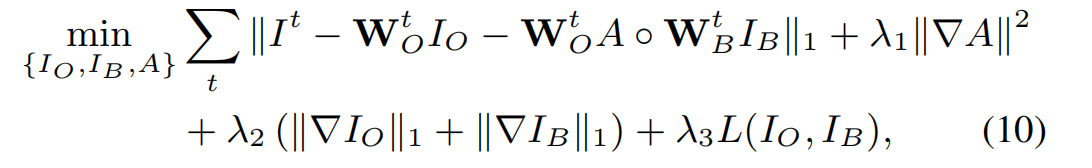
\includegraphics[height=1.5cm,width=10cm]{2022122603.png}
%\caption{图像扭曲}
\end{figure}
约束条件为:
\begin{equation}
0\leq I_O,I_B,A\leq 1
\end{equation}
\end{frame}
\begin{frame}
\frametitle{求解优化问题}
我们应用修正后的迭代重加权最小二乘(IRLS)法\footnote{使用迭代的方式解决带权重的$L^p$范数逼近问题。}解上述方程。原本的IRLS方法是用于求解仅含有$l_1,l_2$范数的无约束最优化问题,因此,我们需要对目标的优化式进行线性化处理。具体而言,我们用
\begin{equation}
xy = x\hat{y}+\hat{x}y-\hat{x}\hat{y}
\end{equation}
进行线性近似,将上式的第一项改写为:
\begin{figure}[!h]
\centering
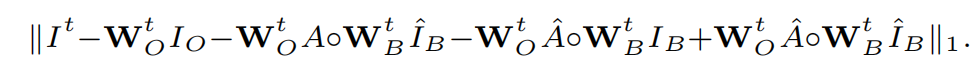
\includegraphics[height=0.8cm,width=8cm]{2022122604.png}
%\caption{图像扭曲}
\end{figure}\pause
同样地,我们将上文中梯度变化独立性的约束条件同样进行线性化处理,得到
\begin{figure}[!h]
\centering
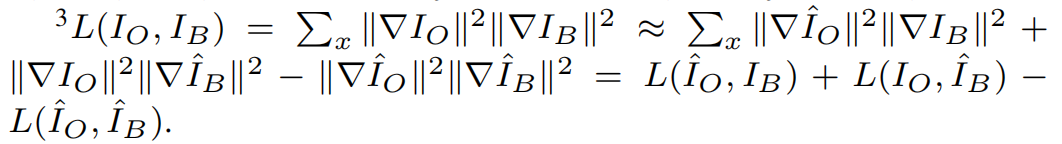
\includegraphics[height=1.2cm,width=8cm]{2022122605.png}
%\caption{图像扭曲}
\end{figure}
\end{frame}
\begin{frame}
\frametitle{求解优化问题}
由于IRLS算法中不能加入约束条件,因此,我们将约束条件
\begin{equation}
0\leq I_O,I_B,A\leq 1
\end{equation}
进行转化。

例如,我们将不等式$0\leq I_B$转化为如下限制,并加入目标函数中:
\begin{equation}
\lambda_p\min(0,I_B)^2
\end{equation}\pause
我们给定$\lambda_p = 10^5$。此时,若$I_B$小于0,随着$I_B$越小,这一项对于整体目标函数的惩罚越大,而$I_B$大于0时,该项为0。对于约束条件中的其他项,用类似的方法处理即可。
\end{frame}
\begin{frame}
\frametitle{求解优化问题}
接下来,只需仿照上述步骤,给定$I_O$,$I_B$,$A$,并用同样的IRLS方法求解$V_O^t$和$V_B^t$即可。\pause

除此以外,我们还需要在使用上述算法前找出运动场。对此,我们首先估计图像的运动情况。本文应用"edge flow"算法,用"Canny edge detector"探测图像边缘像素,其梯度通常较大。再应用离散Markov random field计算每个边缘像素的运动情况。
\end{frame}
\end{document}
